%%%%%%%%%%%%%%%%%%%%%%%%%%%%%%%%%%%%%%%%%
% Masters/Doctoral Thesis 
% LaTeX Template
% Version 2.5 (27/8/17)
%
% This template was downloaded from:
% http://www.LaTeXTemplates.com
%
% Version 2.x major modifications by:
% Vel (vel@latextemplates.com)
%
% This template is based on a template by:
% Steve Gunn (http://users.ecs.soton.ac.uk/srg/softwaretools/document/templates/)
% Sunil Patel (http://www.sunilpatel.co.uk/thesis-template/)
%
% Template license:
% CC BY-NC-SA 3.0 (http://creativecommons.org/licenses/by-nc-sa/3.0/)
%
%%%%%%%%%%%%%%%%%%%%%%%%%%%%%%%%%%%%%%%%%

%----------------------------------------------------------------------------------------
%	PACKAGES AND OTHER DOCUMENT CONFIGURATIONS
%----------------------------------------------------------------------------------------

\documentclass[
11pt, % The default document font size, options: 10pt, 11pt, 12pt
%oneside, % Two side (alternating margins) for binding by default, uncomment to switch to one side
francais, % ngerman for German
singlespacing, % Single line spacing, alternatives: onehalfspacing or doublespacing
%draft, % Uncomment to enable draft mode (no pictures, no links, overfull hboxes indicated)
%nolistspacing, % If the document is onehalfspacing or doublespacing, uncomment this to set spacing in lists to single
%liststotoc, % Uncomment to add the list of figures/tables/etc to the table of contents
%toctotoc, % Uncomment to add the main table of contents to the table of contents
parskip, % Uncomment to add space between paragraphs
%nohyperref, % Uncomment to not load the hyperref package
headsepline, % Uncomment to get a line under the header
%chapterinoneline, % Uncomment to place the chapter title next to the number on one line
%consistentlayout, % Uncomment to change the layout of the declaration, abstract and acknowledgements pages to match the default layout
]{MastersDoctoralThesis} % The class file specifying the document structure

\usepackage[utf8]{inputenc} % Required for inputting international characters
\usepackage[T1]{fontenc} % Output font encoding for international characters

\usepackage{mathpazo} % Use the Palatino font by default

\usepackage[backend=bibtex,style=authoryear,natbib=true]{biblatex} % Use the bibtex backend with the authoryear citation style (which resembles APA)

\addbibresource{example.bib} % The filename of the bibliography

\usepackage[autostyle=true]{csquotes} % Required to generate language-dependent quotes in the bibliography

%----------------------------------------------------------------------------------------
%	MARGIN SETTINGS
%----------------------------------------------------------------------------------------

\geometry{
	paper=a4paper, % Change to letterpaper for US letter
	inner=2.5cm, % Inner margin
	outer=3.8cm, % Outer margin
	bindingoffset=.5cm, % Binding offset
	top=1.5cm, % Top margin
	bottom=1.5cm, % Bottom margin
	%showframe, % Uncomment to show how the type block is set on the page
}

%----------------------------------------------------------------------------------------
%	THESIS INFORMATION
%----------------------------------------------------------------------------------------

\thesistitle{Rapport de Fin Bénin} % Your thesis title, this is used in the title and abstract, print it elsewhere with \ttitle
\supervisor{Dr. James \textsc{Smith}} % Your supervisor's name, this is used in the title page, print it elsewhere with \supname
\examiner{} % Your examiner's name, this is not currently used anywhere in the template, print it elsewhere with \examname
\degree{Doctor of Philosophy} % Your degree name, this is used in the title page and abstract, print it elsewhere with \degreename
\author{John \textsc{Smith}} % Your name, this is used in the title page and abstract, print it elsewhere with \authorname
\addresses{} % Your address, this is not currently used anywhere in the template, print it elsewhere with \addressname

\subject{Biological Sciences} % Your subject area, this is not currently used anywhere in the template, print it elsewhere with \subjectname
\keywords{} % Keywords for your thesis, this is not currently used anywhere in the template, print it elsewhere with \keywordnames
\university{\href{http://www.university.com}{University Name}} % Your university's name and URL, this is used in the title page and abstract, print it elsewhere with \univname
\department{\href{http://department.university.com}{Department or School Name}} % Your department's name and URL, this is used in the title page and abstract, print it elsewhere with \deptname
\group{\href{http://researchgroup.university.com}{Research Group Name}} % Your research group's name and URL, this is used in the title page, print it elsewhere with \groupname
\faculty{\href{http://faculty.university.com}{Faculty Name}} % Your faculty's name and URL, this is used in the title page and abstract, print it elsewhere with \facname

\AtBeginDocument{
\hypersetup{pdftitle=\ttitle} % Set the PDF's title to your title
\hypersetup{pdfauthor=\authorname} % Set the PDF's author to your name
\hypersetup{pdfkeywords=\keywordnames} % Set the PDF's keywords to your keywords
%\hypersetup{urlcolor=blue}
%\hypersetup{citecolor=blue}
}

\begin{document}

\frontmatter % Use roman page numbering style (i, ii, iii, iv...) for the pre-content pages

\pagestyle{plain} % Default to the plain heading style until the thesis style is called for the body content

%----------------------------------------------------------------------------------------
%	TITLE PAGE
%----------------------------------------------------------------------------------------

\begin{titlepage}
\begin{center}

\vspace*{.06\textheight}
{\scshape\LARGE \univname\par}\vspace{1.5cm} % University name
\textsc{\Large Doctoral Thesis}\\[0.5cm] % Thesis type

\HRule \\[0.4cm] % Horizontal line
{\huge \bfseries \ttitle\par}\vspace{0.4cm} % Thesis title
\HRule \\[1.5cm] % Horizontal line
 
\begin{minipage}[t]{0.4\textwidth}
\begin{flushleft} \large
\emph{Author:}\\
\href{http://www.johnsmith.com}{\authorname} % Author name - remove the \href bracket to remove the link
\end{flushleft}
\end{minipage}
\begin{minipage}[t]{0.4\textwidth}
\begin{flushright} \large
\emph{Supervisor:} \\
\href{http://www.jamessmith.com}{\supname} % Supervisor name - remove the \href bracket to remove the link  
\end{flushright}
\end{minipage}\\[3cm]
 
\vfill

\large \textit{A thesis submitted in fulfillment of the requirements\\ for the degree of \degreename}\\[0.3cm] % University requirement text
\textit{in the}\\[0.4cm]
\groupname\\\deptname\\[2cm] % Research group name and department name
 
\vfill

{\large \today}\\[4cm] % Date
%\includegraphics{Logo} % University/department logo - uncomment to place it
 
\vfill
\end{center}
\end{titlepage}

%----------------------------------------------------------------------------------------
%	DECLARATION PAGE
%----------------------------------------------------------------------------------------

\begin{declaration}
\addchaptertocentry{\authorshipname} % Add the declaration to the table of contents
\noindent I, \authorname, declare that this thesis titled, \enquote{\ttitle} and the work presented in it are my own. I confirm that:

\begin{itemize} 
\item This work was done wholly or mainly while in candidature for a research degree at this University.
\item Where any part of this thesis has previously been submitted for a degree or any other qualification at this University or any other institution, this has been clearly stated.
\item Where I have consulted the published work of others, this is always clearly attributed.
\item Where I have quoted from the work of others, the source is always given. With the exception of such quotations, this thesis is entirely my own work.
\item I have acknowledged all main sources of help.
\item Where the thesis is based on work done by myself jointly with others, I have made clear exactly what was done by others and what I have contributed myself.\\
\end{itemize}
 
\noindent Signed:\\
\rule[0.5em]{25em}{0.5pt} % This prints a line for the signature
 
\noindent Date:\\
\rule[0.5em]{25em}{0.5pt} % This prints a line to write the date
\end{declaration}

\cleardoublepage

%----------------------------------------------------------------------------------------
%	QUOTATION PAGE
%----------------------------------------------------------------------------------------

\vspace*{0.2\textheight}

\noindent\enquote{\itshape Thanks to my solid academic training, today I can write hundreds of words on virtually any topic without possessing a shred of information, which is how I got a good job in journalism.}\bigbreak

\hfill Dave Barry

%----------------------------------------------------------------------------------------
%	ABSTRACT PAGE
%----------------------------------------------------------------------------------------

\begin{abstract}
\addchaptertocentry{\abstractname} % Add the abstract to the table of contents
The Thesis Abstract is written here (and usually kept to just this page). The page is kept centered vertically so can expand into the blank space above the title too\ldots
\end{abstract}

%----------------------------------------------------------------------------------------
%	ACKNOWLEDGEMENTS
%----------------------------------------------------------------------------------------

\begin{acknowledgements}
\addchaptertocentry{\acknowledgementname} % Add the acknowledgements to the table of contents
The acknowledgments and the people to thank go here, don't forget to include your project advisor\ldots
\end{acknowledgements}

%----------------------------------------------------------------------------------------
%	LIST OF CONTENTS/FIGURES/TABLES PAGES
%----------------------------------------------------------------------------------------

\tableofcontents % Prints the main table of contents

\listoffigures % Prints the list of figures

\listoftables % Prints the list of tables

%----------------------------------------------------------------------------------------
%	ABBREVIATIONS
%----------------------------------------------------------------------------------------

\begin{abbreviations}{ll} % Include a list of abbreviations (a table of two columns)

\textbf{LAH} & \textbf{L}ist \textbf{A}bbreviations \textbf{H}ere\\
\textbf{WSF} & \textbf{W}hat (it) \textbf{S}tands \textbf{F}or\\

\end{abbreviations}

%----------------------------------------------------------------------------------------
%	PHYSICAL CONSTANTS/OTHER DEFINITIONS
%----------------------------------------------------------------------------------------

\begin{constants}{lr@{${}={}$}l} % The list of physical constants is a three column table

% The \SI{}{} command is provided by the siunitx package, see its documentation for instructions on how to use it

Speed of Light & $c_{0}$ & \SI{2.99792458e8}{\meter\per\second} (exact)\\
%Constant Name & $Symbol$ & $Constant Value$ with units\\

\end{constants}

%----------------------------------------------------------------------------------------
%	SYMBOLS
%----------------------------------------------------------------------------------------

\begin{symbols}{lll} % Include a list of Symbols (a three column table)

$a$ & distance & \si{\meter} \\
$P$ & power & \si{\watt} (\si{\joule\per\second}) \\
%Symbol & Name & Unit \\

\addlinespace % Gap to separate the Roman symbols from the Greek

$\omega$ & angular frequency & \si{\radian} \\

\end{symbols}

%----------------------------------------------------------------------------------------
%	DEDICATION
%----------------------------------------------------------------------------------------

\dedicatory{For/Dedicated to/To my\ldots} 

%----------------------------------------------------------------------------------------
%	THESIS CONTENT - CHAPTERS
%----------------------------------------------------------------------------------------

\mainmatter % Begin numeric (1,2,3...) page numbering

\pagestyle{thesis} % Return the page headers back to the "thesis" style

% Include the chapters of the thesis as separate files from the Chapters folder
% Uncomment the lines as you write the chapters

% Chapter 1

\chapter{Chapter Title Here} % Main chapter title


%\chapter{Cadre contextuel}
\section{Problématique}
Depuis l'avènement du commerce électronique, de nombreuses plate-formes offrant le service de vente en ligne ont vu le jour. La multiplication de ces plates-formes a complètement changé le comportement de l’internaute : depuis son ordinateur, sa tablette ou son Smartphone, ce dernier peut acheter en ligne les produits qu'il désire sur la plate-forme qui lui convient. 

En France cette activité à augmenter de manière très importante en terme de chiffre d'affaires plus de 20 Milliards d'euro en 2012 avec un taux d'accroissement annuel de 20 \%. Vu l'importance de ce commerce dans les pays du nord, il est regrettable de constater que cette activité reste peu développée en Afrique et particulièrement inexistantes au Bénin. Les quelques plates-formes qui y ont vu le jour, sont réalisées à base de solutions pré-conçues, solutions qui généralement, ne répondent pas aux exigences et besoins du marché local à cause des solutions de paiement qu'elles proposent. 

Ainsi, pour palier à ce problème et faire de l’e-commerce une activité effective au Bénin, il est impératif de développer des plate-formes de vente en ligne modernes et flexibles qui répondent aux exigences du marché local et qui respectent les normes sécuritaires.

\section{Environnement économique global}
Le commerce électronique est l'un des facteurs phares pour le développement de l'économie. En effet, avec l'apparition du commerce électronique les relations entres vendeurs et acheteurs ont connu de grandes changement. L'e-commerce a surmonté l'handicape structurel de la distanciation physique et de prestation différée.
Il a un atout important sur l'environnement économique, les ménages jouissent d'une nouvelle liberté, en pratiquant désormais ce commerce qui offre de nombreux services publics en ligne. Ce commerce poursuit une croissance d'extension vers la communication multimédia.

L'e-commerce est une activité qui ne fait que croître depuis 2010. En 2017, les ventes en ligne sur les plates-formes d'e-commerce se sont élevées à 2.304 milliards de dollars américain.

\section{Environnement économique local}
En 2017, les ventes en ligne en moyen-orient et en Afrique s'élèvent à seulement 16.651 millions de dollars américain, soit moins de 1\% des ventes mondiales. Ces statistiques sont énormes et montrent à quel point l'Afrique est en traîne dans ce domaine. Ce faible pourcentage est essentiellement dû à l'absence de moyens de paiement sécurisés. Cependant, avec la multiplication des moyens de paiement mobiles, l'Afrique peut espérer une croissance en e-commerce si toutefois des plates-formes d'e-commerce sécurisées, intégrant ces nouveaux moyens de paiement, voyaient le jour.
 
%\chapter{Plate-forme d'e-commerce}
	\section{Concepts clés}
\subsection{Le commerce électronique ou e-commerce}
Le commerce électronique regroupe l’ensemble des transactions commerciales s’opérant à distance par le biais d’interfaces électroniques et digitales à partir des différents types de terminaux (Ordinateurs, tablettes, smartphones, consoles, TV connectées).

\subsection{Le Marché virtuel}
Le marché virtuel est un marché qui le plus souvent à une dimension internationale et qui sont plutôt des évènements permanents. Il permet aux investisseurs de se présenter, d’entrer en contact facilement, de faire connaitre leurs besoins en matière de développement et de trouver des partenaires pour satisfaire ces besoins.

\subsection{E-Vendeur}
E-vendeur est un vendeur en ligne, il est chargé de rendre disponible ses produits, donner ces caractéristiques et d'ajouter le prix de chacun de ces articles dans le but de les vendre aux clients actuels.

\subsection{E-Acheteur}
Les e-acheteurs sont fortement demandeurs d’offres personnalisées, notamment parmi les adhérents à des programmes de fidélisation. L'e-acheteur à un rôle très important. En effet, il se charge de consulter les produits en ligne, sélection, paie, et reçoit en toute sécurité les produits commander.

\subsection{E-Boutique}
E-boutique est une boutique de vente de produits, des biens et services en ligne. Grâce à une boutique en ligne, on peut choisir et payer des articles comme dans un magasin réel. Pour acheter un produit dans cette boutique virtuelle, il suffit de choisir les produits désirés puis de les mettre dans un panier. L’acheteur peut remplir un bon et payer sa commande par carte bancaire ou par un autre moyen de paiement. La commande sera livrée en fonction du choix de l’internaute et selon les modalités définies par le responsable de la boutique.


\section{Approche et démarche d'analyse}

Les auteurs d’UML préconisent l’utilisation d'une démarche itérative, incrémentale et guidée par les besoins des utilisateurs du'un système dans la réalisation d’une application informatique.

La méthode Agile Scrum est la méthode utilisée pour cette réalisation. Cette méthode de réalisation du projet est basée sur des indications. Avec cette méthode, un processus est défini et suivi pour la réalisation.


\subsection{Méthode Agile Scrum}
Cette méthode agile  permet la réalisation d'un projets complexe en favorisant l'interaction avec les membres de l'équipe et les managers, la collaboration du client et la réactivité face aux changement. Elle permet de produire une plus grande 
valeur ajoutée dans la durée la plus  courte. Elle est une approche itérative et incrémentable, qui est menée dans un esprit collaboratif. Elle génère un produit de haute qualité tout en prenant en compte l’évolution des besoins des clients.


Scrum est la méthode Agile la plus utilisée de nos jours. En bref, elle définit des rôles: le Scrum Master, le Product Owner et l’équipe de développement, dicte la réitération de sprints, de production à durée limitée à la fin desquels des incréments fonctionnels de logiciel sont livrés et met en place des artefacts (le carnet de produit, le carnet de sprint, les graphiques d’avancement) ainsi que des cérémonies (planification de sprint, mêlée quotidienne, revue et rétrospective).

Elle implique l’auto-organisation des équipes et permet beaucoup plus la réactivité pour s’adapter aux besoins (parfois changeants) du client. Elle sous-entend aussi l’application de principes Agiles, soit la transparence, la simplicité et la collaboration.
La méthode Scrum soutient la livraison rapide et régulière de fonctionnalités à haute valeur ajoutée.

\subsubsection{Backlog}
Le Backlog Sprint est l’ensemble des éléments sélectionnés pour le Sprint plus un plan pour livrer l’incrément du produit et réaliser l’objectif du Sprint. Le Backlog Sprint est une prévision que l’équipe de développement fait de la fonctionnalité qui sera présente dans le prochain incrément et le travail nécessaire pour livrer cette fonctionnalité dans un incrément «Fini»
Le Backlog Sprint rend visible tout le travail que l'équipe de développement identifie comme nécessaire pour atteindre l'objectif du Sprint.
Le Backlog Sprint est un plan suffisamment détaillé pour que la progression soit compréhensible lors de la mêlée quotidienne.

\subsubsection{Items}
Les items d'un backlog sont les différents éléments constitutifs d'un backlog produit.Le Backlog Produit est une liste ordonnée de tous les éléments identifiés comme nécessaires au produit. Il constitue l’unique source d'exigences pour tout changement à apporter au produit. Le Backlog Produit liste toutes les fonctionnalités, les fonctions, les exigences, les améliorations et les corrections qui constituent des modifications à apporter au produit dans les versions futures. Les éléments du backlog produit se composent d'une description, d'un ordre, d'une
estimation et d'une valeur. Les éléments du backlog produit incluent souvent des descriptions du test qui prouveront leur complétude lorsqu’ils sont «Finis ».

\subsubsection{Sprint}
Un Sprint est défini pour réaliser un objectif, la définition des fonctionnalités de l’activité à développer, la conception et le plan flexible qui guidera le développement, la durée du sprint est limitée à  (moins d’un mois).
Il contient et est constitué de la planification du Sprint, des mêlées quotidienne, des activités de développement, de la revue du Sprint et de la rétrospective du Sprint.
Le sprint a un objectif fixe auquel est associée une liste d’éléments du Product backlog, ce but est sans changements qui le remettent en cause. Les objectifs de qualités sont maintenus.
Sprints amènent de la prévisibilité en forçant une inspection et adaptation du progrès vers l’atteinte d’un objectif au moins mensuellement.

\subsubsection{La Mêlée}
La mêlée quotidienne, encore appelé daily scrum est un événement limité à 15 minutes au cours duquel l'équipe de développement synchronise ses activités et crée un plan pour les prochaine heures.
Elle réunit tous les membres de l’équipe et permet d’examiner les tâches en cours et les difficultés rencontrées.
Les mêlées quotidiennes améliorent la communication, éliminent les autres réunions, identifient
les obstacles qui perturbent le développement afin qu'ils soient éliminés, mettent en avant et encouragent la prise de décision rapide tout en améliorant le niveau de connaissance au sein de l’équipe de développement. Il s’agit d’un point clé d’inspection et d’adaptation.

	\section{Analyse et Conception}
Pour faire face à la complexité croissante des systèmes d’informations, de nouvelles méthodes et outils ont été créés.Dans le cadre de notre analyse, c’est un langage appelé UML (Unified Modeling Language) qui est celui retenu pour la modélisation du système à mettre en place.

En effet l'UML se traduit par un Langage de modélisation unifié. Il s’agit d’un langage visuel constitué d’un ensemble de schémas, appelés diagrammes, donnant chacun une vision différente du système à traiter. L'UML nous fournit donc des diagrammes pour représenter l’application à développer: son fonctionnement, sa mise en route, les actions susceptibles d’être effectuées par l’application, etc. L'UML, est un langage basé sur le concept de la Programmation Orientée Objet. Il ne préconise aucune démarche, ce n’est donc en aucun cas une méthode. Chacun est libre d’utiliser les types de diagramme qu’il souhaite, dans l’ordre qu’il veut. Il suffit que les diagrammes réalisés soient cohérents entre eux, avant de passer à la réalisation de l’application.

\subsection{Étude des Processus Métier}
Les processus métier constituent le mécanisme principal par lequel les services d'entreprise sont intégrés. C'est un ensemble d'activité visant à atteindre un objectif particulier d'une entreprise. Ce processus métier apporte une vision du métier réel, et constitue un excellent instrument de formalisation et d'analyse dans la construction des systèmes.
Dans le cas d'Oqenyite, les processus métier sont les suivants créer boutique, gérer catalogue en ligne, effectuer commande.


\subsubsection* {Gérer boutique}
Le processus gérer un boutique consiste à  
modifier les différents produits de la boutique: ajouter supprimer classer les produits par catégorie.  Après ça, il a la possibilité d’exposer ces produits, de donner ces caractéristiques et afficher les prix selon la catégorie de chaque produit. 

\subsubsection*{Gérer catalogue}
Ici le vendeur expose ces produits par catégorie en précisant les caractéristiques suivi des détails tout en mentionnant le prix de chaque produits, les mets en ligne.


\subsubsection*{Effectuer commande}
Pour faire des achats ou pour passer une commande le visiteur ou l'acheteur avant de voir les produit disponible sur la plate-forme d'oqenyite doit se connecter c'est à dire avoir un compte. Une fois connecté l'acheteur a la possibilité de consulter tous les produit existant sur la plate forme, voir leurs caractéristique, ainsi que le prix de chaque produits. Maintenant il fait le choix des produits désirés les ajoutent au panier et passe sa commande.



\subsubsection*{Gérer livraison}
La gestion de la livraison se fait comme suit, l'acheteur après avoir validation du panier choisir son adresse de livraison, si il n'a pas adresse de livraison, il a la possibilité d'ajouter son adresse. Il choisit ensuite le mode de livraison entre livraison (express ou classique). Il sélectionne un moyen de paiement et effectue le paiement.

Le processus métier nous conduit à la réalisation des digrammes d'activités et d'objet de flux.


\subsection{Diagramme d'Activité et Objet de Flux}

Le diagramme d’activité est attaché à une catégorie de classe et décrit le déroulement des activités de cette catégorie. Il indique la part prise par chaque objet dans
l’exécution d’un travail.

Objet de flux est un connecteur avec une pointe de flèche dénotant la direction ou on passe l’objet. Il doit avoir un objet sur au moins une de ses fins. 
Ce diagramme d'activité sera lié au processus effectuer commende.

\textbf{Image manquante ici !!!!!!!!!!!!!!!!}

%\begin{minipage}{1\textwidth}
%	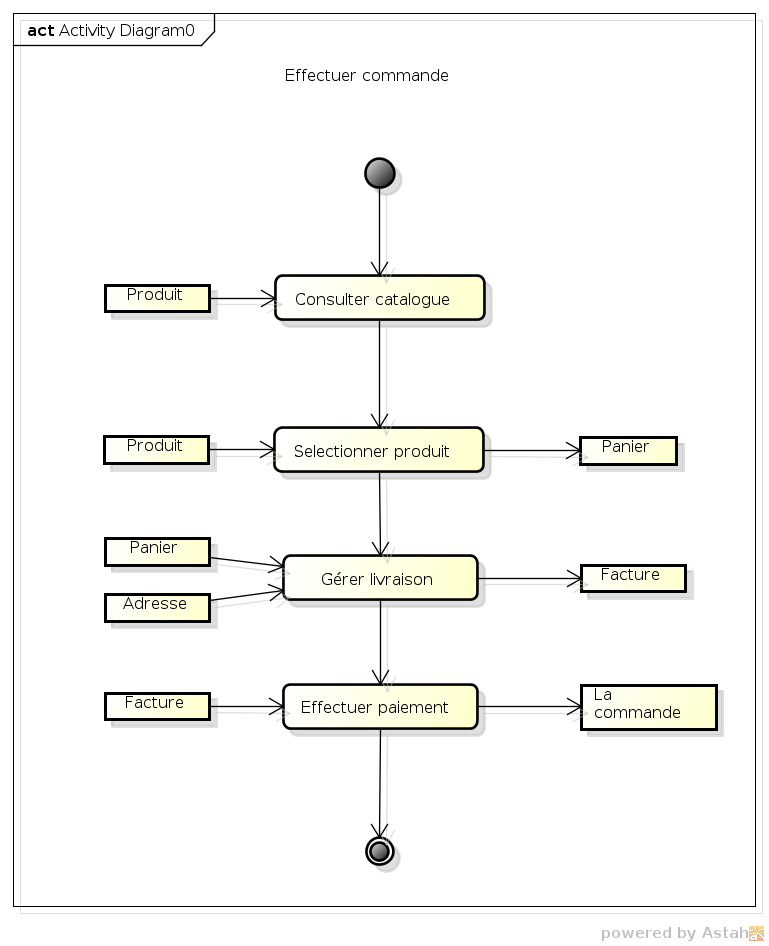
\includegraphics[width=0.7\linewidth]{mama/images/Effectuer}
%	\label{fig:Effectuer}
%\end{minipage}
%\hspace*{\stretch{1}}

Le diagramme d’activité est un Diagramme associé à un objet particulier ou à un ensemble d’objets, qui illustre les flux entre les activités et les actions. Il permet de représenter graphiquement le déroulement d’un cas d’utilisation métier sur les commandes.



\subsection{Cas d'Utilisation Métier}


Le rôle du diagramme de cas d’utilisation métier est de recueillir, d’analyser et d’organiser les besoins, ainsi que de recenser les grandes fonctionnalités d’un système. 

%\begin{minipage}{1,1\textwidth}
%	
%	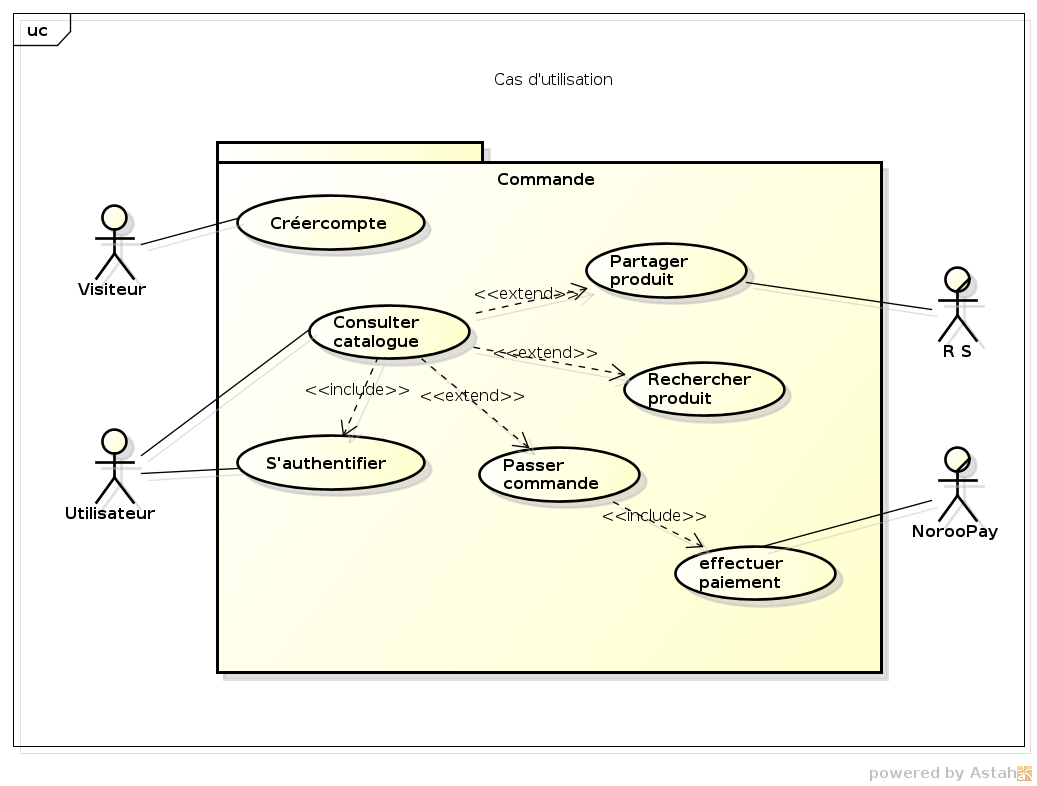
\includegraphics[width=0.7\linewidth]{mama/images/utilisation}
%	\label{fig:utilisation}
%\end{minipage}
%\hspace*{\stretch{1}}

\textbf{Image manquante ici !!!!!!!!!!!!!!!!}


\subsection{Diagramme de Séquence}

le diagramme de séquence est un diagramme d’interaction qui expose en détail
la façon dont les opérations sont effectuées: quels messages sont envoyés et quand ils le sont. Les diagrammes de séquences sont organisés en fonction du temps qui s’écoule au fur et à mesure que nous parcourons la page. Les objets impliqués dans l’opération sont répertoriés de gauche, à droite en fonction du moment où ils prennent part dans la séquence.

\textbf{Image manquante ici !!!!!!!!!!!!!!!!}
%\begin{minipage}{0,8\textwidth}
%	\includegraphics[width=0.7\linewidth]{mama/images/séquence}
%\end{minipage}
%\hspace*{\stretch{1}}


\subsection*{Diagramme de classes}

Le diagramme de classes exprime la structure statique du système en termes de classes et de relations entre ces classes. L’intérêt du diagramme de classe est de modéliser les entités du système d’information.
Le diagramme de classe permet de représenter l’ensemble des informations finalisées qui sont gérées par le domaine. Ces informations sont structurées, c’est-à-dire qu’elles sont regroupées dans des classes. Ce
diagramme met en évidence d’éventuelles relations entre ces classes.
%
%\begin{minipage}{1\textwidth}
%	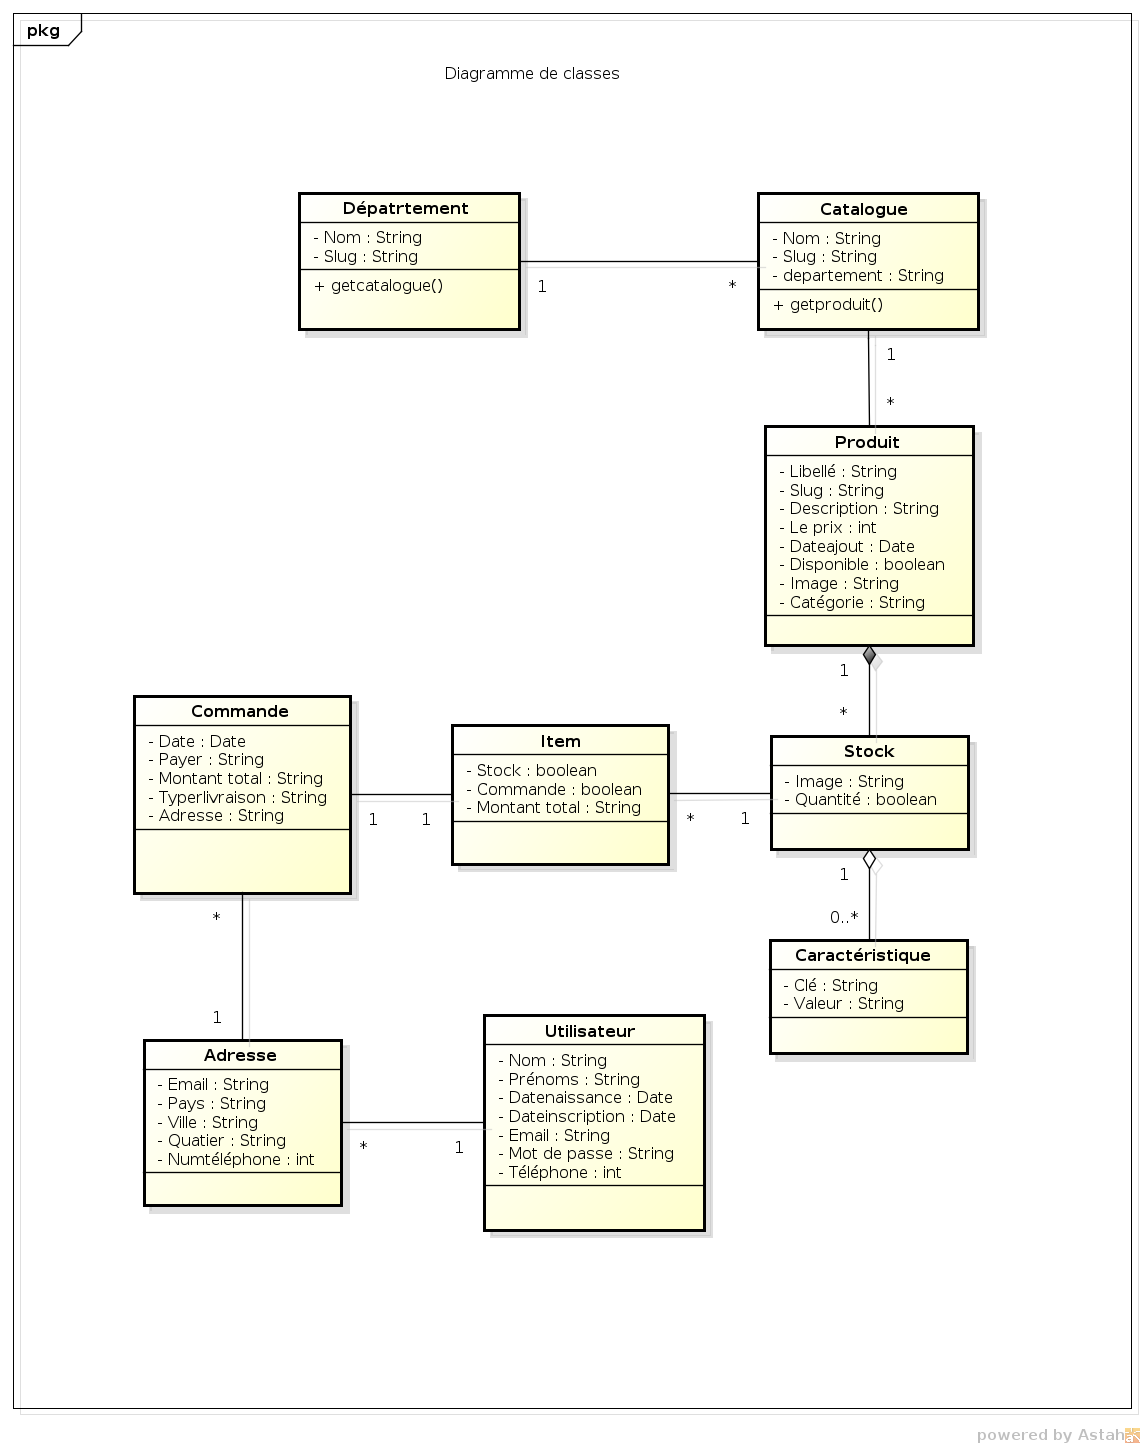
\includegraphics[width=0.7\linewidth]{mama/images/classes}
%\end{minipage}
%\hspace*{\stretch{1}}
\textbf{Image manquante ici !!!!!!!!!!!!!!!!}


Chaque classe se décrit par les données et les traitements dont elle est responsable pour elle-même et vis-à-vis des autres classes. Les traitements sont matérialisés par des opérations.


\subsection{Diagramme de Déploiement}

Les diagrammes de déploiement montrent la disposition physique des différents matériels appelés nœuds(ordinateurs, périphériques, réseaux, systèmes de stockage...) qui entrent dans la composition d’un système et la répartition des instances de composants, processus et objets qui vivent sur ces matériels. Les diagrammes de déploiement sont donc très utiles pour modéliser l’architecture physique d’un système.

%\begin{minipage}{1,2\textwidth}
%	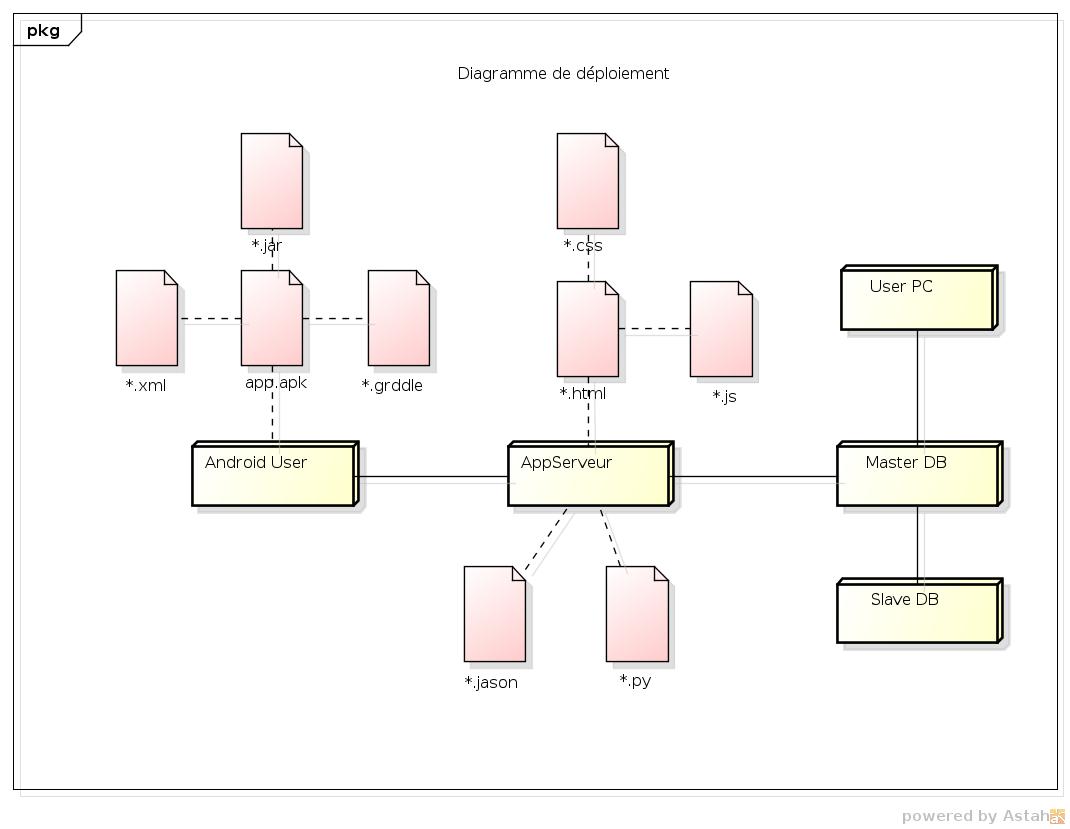
\includegraphics[width=0.7\linewidth]{mama/images/Deployment}
%	\label{fig:deployment}
%\end{minipage}
%\hspace*{\stretch{1}}
\textbf{Image manquante ici !!!!!!!!!!!!!!!!}

C'est en partant de ces diagrammes qu'on écrit le code informatique pour répondre aux besoins des utilisateurs.








%\include{Chapters/Chapter4} 
%\include{Chapters/Chapter5} 

%----------------------------------------------------------------------------------------
%	THESIS CONTENT - APPENDICES
%----------------------------------------------------------------------------------------

\appendix % Cue to tell LaTeX that the following "chapters" are Appendices

% Include the appendices of the thesis as separate files from the Appendices folder
% Uncomment the lines as you write the Appendices

% Appendix A


%\include{Appendices/AppendixB}
%\include{Appendices/AppendixC}

%----------------------------------------------------------------------------------------
%	BIBLIOGRAPHY
%----------------------------------------------------------------------------------------

\printbibliography[heading=bibintoc]

%----------------------------------------------------------------------------------------

\end{document}  
